\section{Overview of Experiments}

Four evaluation phases were executed against frozen code with provenance recording (git commit \texttt{7e08016}, CPU-only Intel i3-6006U, no GPU). Phase~1 probed public datasets (CDnet-2014, UCF-Crime; 514 sampled inferences, 0 skipped/failed, 88.7\,s). Phase~2 calibrated the risk score over 64 labelled seconds (473 inferences, 176.1\,s) under Leave-One-Video-Out. Phase~3 tested forensic integrity over 470 frames per case. Phase~4 ran the locked baseline comparison (24 encodes: 16 primary + 8 control; $\approx$ 3.5 hours wall-clock, 9764\,s). This chapter reports each phase in RESULT $\rightarrow$ EVIDENCE $\rightarrow$ INTERPRETATION $\rightarrow$ LIMITATION order. Numbers below are taken verbatim from \texttt{experiments/phase{1,2,3,4}\_*/} CSV and JSON evidence files.

\section{Phase 1: Public-Dataset Observations}

\subsection{CDnet-2014}

\begin{table}[H]
\centering
\caption{Phase~1 CDnet-2014 results (confidence 0.30, every 30th frame, hour fixed to 14)}
\label{tab:phase1-cdnet}
\begin{tabular}{|l|c|c|c|c|c|}
\hline
\textbf{Scene} & \textbf{Samples} & \textbf{Risk mean $\pm$ std} & \textbf{Detect.\ rate} & \textbf{Agreement} & \textbf{TP/FP/FN} \\
\hline
highway & 57 (41 in ROI) & 0.563 $\pm$ 0.234 & 0.983 & 0.976 & 40/0/1 \\
pedestrians & 37 (27 in ROI) & 0.492 $\pm$ 0.264 & 1.000 & 0.778 & 21/6/0 \\
streetCornerAtNight & 174 (147 in ROI) & 0.024 $\pm$ 0.056 & 0.121 & 0.803 & 10/8/21\footnotemark \\
\hline
\end{tabular}
\end{table}
\footnotetext{TN = 108 for streetCornerAtNight; TN = 0 for highway and pedestrians (temporal ROI contains motion throughout).}

RESULT: On highway, the risk score averaged $0.563 \pm 0.234$ with agreement 0.976 (40 TP, 0 FP, 1 FN). EVIDENCE: \texttt{experiments/phase1\_public/cdnet\_scene\_results.csv}. INTERPRETATION: where persistent person/vehicle activity fills the temporal ROI, detection presence aligns closely with ground-truth motion and the risk score sits in the ALERT band. LIMITATION: the temporal ROI of this scene contains almost no negative samples (TN = 0), so agreement here measures recall-like behaviour, not balanced accuracy; the hour was fixed to 14 for comparability, which is artificial for the night scene.

RESULT: On pedestrians, risk averaged $0.492 \pm 0.264$ with agreement 0.778 (21 TP, 6 FP, 0 FN). INTERPRETATION: the detector fires reliably (detection rate 1.0) but produces false positives relative to the motion ground truth, consistent with a detector-presence signal that is broader than pixel-motion truth. LIMITATION: same single-class-positive caveat as highway.

RESULT: On streetCornerAtNight, risk averaged $0.024 \pm 0.056$ with detection rate 0.121 and agreement 0.803 (10 TP, 108 TN, 8 FP, 21 FN). INTERPRETATION: under night conditions with the hour artificially fixed to 14 (no night bonus) and CPU-only YOLOv8n at 640-pixel width, the detector largely misses the scene's motion content; the high TN count sustains agreement despite 21 false negatives. LIMITATION: this scene exposes the detector's night weakness and the hour-fixing limitation simultaneously; it must not be read as a general night-performance claim.

\subsection{UCF-Crime}

\begin{table}[H]
\centering
\caption{Phase~1 UCF-Crime results (clip-level labels; Fighting002 training-split, annotation pack absent)}
\label{tab:phase1-ucf}
\begin{tabular}{|l|c|c|c|c|}
\hline
\textbf{Video} & \textbf{Label} & \textbf{Risk mean $\pm$ std} & \textbf{Detect.\ rate} & \textbf{Samples} \\
\hline
Normal\_015 & normal & 0.467 $\pm$ 0.360 & 0.938 & 16 \\
Normal\_050 & normal & 0.994 $\pm$ 0.033 & 1.000 & 140 \\
Fighting002 & abnormal & 0.068 $\pm$ 0.135 & 0.311 & 90 \\
\hline
\end{tabular}
\end{table}

RESULT: Normal\_050 (normal label) scored risk $\approx$ 0.994 while Fighting002 (abnormal label) scored risk $\approx$ 0.068 with detection rate 0.311. EVIDENCE: \texttt{experiments/phase1\_public/ucf\_video\_results.csv} and \texttt{annotation\_check.json}. INTERPRETATION: this inversion is expected once the two quantities are correctly understood---the heuristic risk score measures detected-object/ROI importance (crowded normal scenes score highly), whereas UCF-Crime anomaly labels annotate video-level abnormal events (a distant fight with few confident detections scores lowly). High risk therefore does \textit{not} mean anomaly, and the two concepts are not equivalent. LIMITATION: Fighting002 comes from the training split with the annotation pack unavailable, so only the clip-level label was used and no frame-level ground-truth evaluation is claimed; Burglary001 was not evaluated at all because its canonical file could not be verified in isolation.

\section{Phase 2: Calibration Analysis}

\subsection{Label Basis}

The calibration set comprises 64 seconds (17 positive, 47 negative) from \texttt{day\_person}, \texttt{day\_empty}, and \texttt{night} (\texttt{evaluation/labels/*.csv}), manually/visually verified with YOLO as assistance only; one night false positive at second 12 (a traffic cone) was corrected. All 17 positives originate from a single video (\texttt{day\_person}). The fitted model is $P(y{=}1)=\mathrm{sigmoid}(a+b\cdot\mathrm{risk})$ on frozen per-second mean risk.

\subsection{Leave-One-Video-Out Behaviour}

\begin{table}[H]
\centering
\caption{Phase~2 Leave-One-Video-Out folds (AUC undefined for single-class tests by construction)}
\label{tab:phase2-lovo}
\begin{tabular}{|l|l|c|c|c|}
\hline
\textbf{Fold} & \textbf{Test clip} & \textbf{n train/test} & \textbf{Outcome} & \textbf{Brier} \\
\hline
F1 & day\_empty (all negative) & 38 / 26 & specificity only, no AUC & 0.0536 \\
F2 & night (all negative) & 43 / 21 & specificity only, no AUC & 0.1422 \\
F3 & day\_person (all positive) & 47 / 17 & degenerate: 0-positive train, no fit & --- \\
FULL & all (descriptive) & 64 / 64 & apparent metrics only & 0.0878 \\
\hline
\end{tabular}
\end{table}

RESULT: F1 and F2 test folds are single-class (all negative), so ROC-AUC is mathematically undefined and was not reported; F1 achieved specificity 1.0 (26/26 TN) while F2 showed 18 false positives against 3 true negatives at its fitted threshold. F3 could not be fit at all because its training set contained zero positives. EVIDENCE: \texttt{experiments/phase2\_calibration/calibration\_results.json}, \texttt{calibration\_metrics.csv}. INTERPRETATION: the label distribution (positives concentrated in one video) makes independent generalization untestable under LOVO; the folds diagnose the data limitation rather than the model. LIMITATION: no fold constitutes an independent generalization test.

\subsection{Full-Set Descriptive Metrics}

RESULT: The full-set descriptive fit ($a=-2.0055$, $b=3.4353$, threshold 0.35) yields AUC $\approx$ 0.9962, F1 $\approx$ 0.919, precision $\approx$ 0.850, recall = 1.00, specificity $\approx$ 0.936, PR-AUC $\approx$ 0.990, and Brier $\approx$ 0.088 (baseline frozen-risk at 0.30: F1 0.850, Brier 0.064). EVIDENCE: \texttt{calibration\_metrics.csv}, \texttt{coefficients.csv}, \texttt{threshold\_grid.csv}. INTERPRETATION: within-sample, per-second mean risk separates the 64 labelled seconds well, and the fitted logistic improves over the frozen 0.30 threshold on F1. LIMITATION: these metrics are apparent/descriptive/in-sample by construction---they reuse the training data as the test data and all positives come from one video---so they establish separability of this small labelled set only, and must never be headlined as 99.6\% AUC, 100\% recall, or perfect detection without that qualification.

\begin{figure}[H]
\centering
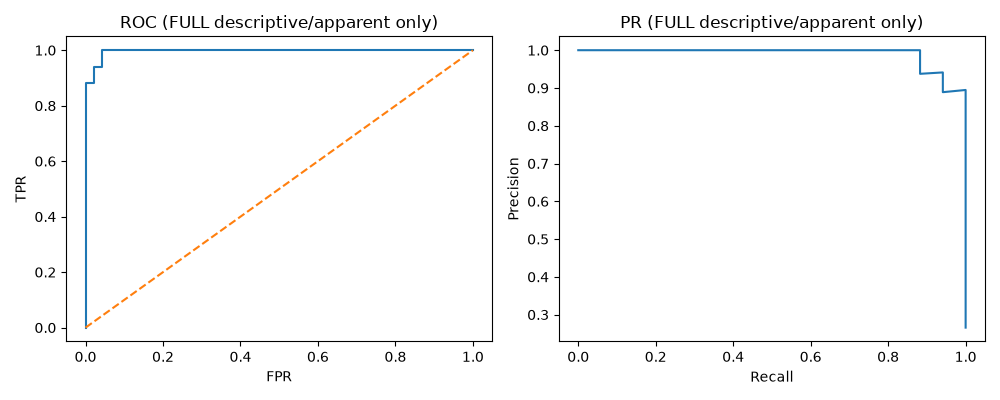
\includegraphics[width=0.85\textwidth]{figures/phase2_roc_pr.png}
\caption{Phase~2 full-set apparent ROC and precision--recall curves (in-sample, descriptive only; not generalization evidence). Source: \texttt{experiments/phase2\_calibration/roc\_pr\_full\_apparent.png}.}
\label{fig:phase2-roc}
\end{figure}

\begin{figure}[H]
\centering
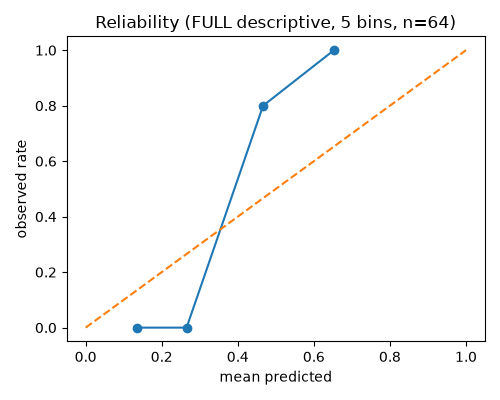
\includegraphics[width=0.85\textwidth]{figures/phase2_reliability.png}
\caption{Phase~2 reliability diagram for the full-set descriptive fit ($n=64$). Source: \texttt{experiments/phase2\_calibration/reliability\_full.png}.}
\label{fig:phase2-rel}
\end{figure}

\section{Phase 3: Forensic Integrity}

\begin{table}[H]
\centering
\caption{Phase~3 forensic cases (470 frames; source \texttt{data/thesis\_clips/motion\_only.mp4})}
\label{tab:phase3}
\begin{tabular}{|l|c|c|c|c|}
\hline
\textbf{Case} & \textbf{Expected} & \textbf{Verdict} & \textbf{Detail} & \textbf{Met} \\
\hline
original & PASS & PASS & 470/470 pass & Yes \\
clean\_control & PASS & PASS & 470/470 pass & Yes \\
recompressed\_vs\_original & FAIL & FAIL & 470/470 mismatch from ev\_00001.jpg & Yes \\
recompressed\_own\_manifest & PASS & PASS & 470/470 pass & Yes \\
tampered\_vs\_pristine & FAIL & FAIL & 1 missing, 4 hash, 416 chain; first ev\_00050.jpg & Yes \\
\hline
\end{tabular}
\end{table}

RESULT: All five cases met their pre-registered expectations. Direct tamper localization scored 5/5 detected (precision 1.0, recall 1.0) with zero false alarms in clean cases. EVIDENCE: \texttt{experiments/phase3\_forensics/cases.csv}, \texttt{localization.csv}, \texttt{custody.json}. INTERPRETATION: the hash chain behaves as an exact-byte tamper-evident mechanism---it passes untouched evidence (including a freshly generated manifest over recompressed content) and fails loudly on any byte-level alteration, with cascade breaks that localize the first tamper point. The recompression FAIL is a predicted bound of exact-byte hashing, not an experiment failure. LIMITATION: this demonstrates exact-byte/hash-chain integrity behaviour only; it establishes no legal admissibility, court-grade validity, certification, standards compliance, or real-world chain-of-custody sufficiency, and only the listed tampering operations were tested.

\begin{figure}[H]
\centering
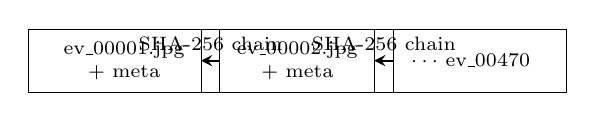
\begin{tikzpicture}[
  node distance=2.2cm, auto,
  file/.style={rectangle, draw, text width=2.2cm, minimum height=0.8cm, align=center, font=\scriptsize},
  arrow/.style={->, >=stealth, thick, font=\scriptsize}
]
\node[file] (f1) {ev\_00001.jpg + meta};
\node[file, right of=f1] (f2) {ev\_00002.jpg + meta};
\node[file, right of=f2] (f3) {$\cdots$ ev\_00470};
\draw[arrow] (f1) -- node[above] {SHA-256 chain} (f2);
\draw[arrow] (f2) -- node[above] {SHA-256 chain} (f3);
\end{tikzpicture}
\caption{Tamper-evident hash-chain structure: each manifest entry binds the file digest to the previous link from a GENESIS anchor. Any deletion, pixel edit, or sidecar modification breaks its own link and every downstream link.}
\label{fig:hashchain}
\end{figure}

[FIGURE PLACEHOLDER --- Figure~7.5: Tampering example (blackout box on frames 50/100/150). What to show: one tampered frame with the (500,200,200,200) blackout region marked. Purpose: concrete illustration of the tested tamper operations. Placement: after Section~7.3. Suggested size: 60--70\% of text width. Source: \texttt{experiments/phase3\_forensics/evidence\_tampered/}. Status: AVAILABLE --- NEEDS FORMATTING (export single frame with annotation).]

\section{Phase 4: Controlled Baseline Comparison}

\subsection{Rate--Distortion Behaviour}

RESULT: On the primary clip (motion\_only, 720p, 235 frames, libx265), measured operating points were: uniform $\approx$ 495/840/1520/2832 kbps with PSNR $\approx$ 36.5/39.4/42.3/45.2; ROI-QP $\approx$ 360/721/1434/2806 kbps with PSNR $\approx$ 33.5/35.5/37.1/38.4; foreground/background split $\approx$ 382/770/1540/3085 kbps with PSNR $\approx$ 13.4--13.5 flat; proposed adaptive ROI $\approx$ 355/710/1399/2754 kbps with PSNR $\approx$ 33.8/36.2/38.1/39.7. ROI-PSNR ranges were 31.5--41.6 (uniform), 28.8--36.6 (ROI-QP), 20.9--21.5 (split), and 28.7--37.0 (proposed); background PSNR ranges were 38.4--46.4 (uniform), 35.5--39.1 (ROI-QP), $\approx$ 12.8 flat (split), and 35.9--40.8 (proposed). EVIDENCE: \texttt{experiments/phase4\_sota/roi\_metrics.csv}, \texttt{runs.csv}. INTERPRETATION: the ROI-based methods operate at lower bitrates than uniform at the same targets (they discard background information by design) but at lower global and ROI fidelity on this sequence; the foreground/background split's flat $\approx$ 13.5 dB PSNR is a negative result caused by its frozen-frame-0 background assumption being inappropriate for the moving-camera clip. LIMITATION: conclusions are confined to the evaluated configuration (single primary motion clip, CPU libx265 medium, stated background scales).

\begin{figure}[H]
\centering
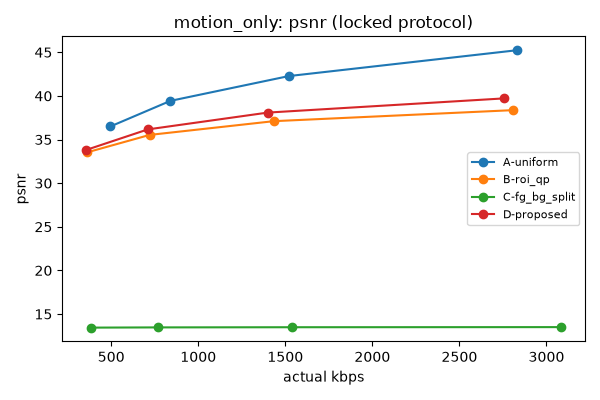
\includegraphics[width=0.85\textwidth]{figures/phase4_rd_psnr.png}
\caption{Phase~4 global rate--distortion curves (PSNR vs.\ actual bitrate, motion\_only, libx265). Source: \texttt{experiments/phase4\_sota/rd\_psnr.png}.}
\label{fig:rd-psnr}
\end{figure}

\begin{figure}[H]
\centering
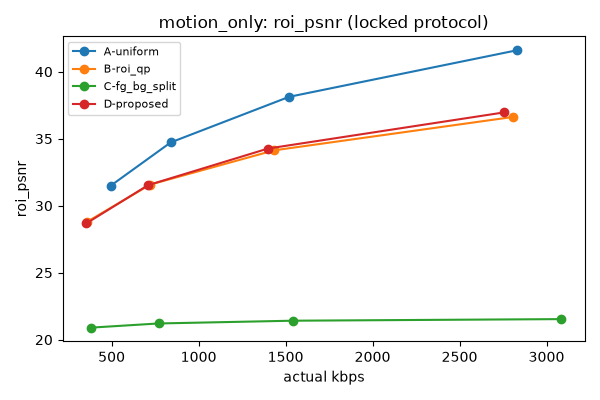
\includegraphics[width=0.85\textwidth]{figures/phase4_rd_roi.png}
\caption{Phase~4 ROI rate--distortion curves (ROI-PSNR vs.\ actual bitrate). Source: \texttt{experiments/phase4\_sota/rd\_roi.png}.}
\label{fig:rd-roi}
\end{figure}

\begin{figure}[H]
\centering
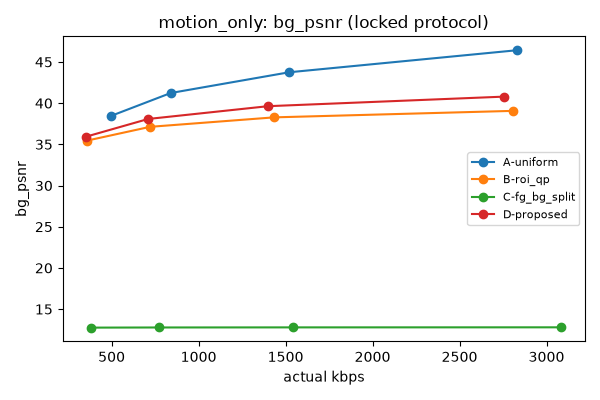
\includegraphics[width=0.85\textwidth]{figures/phase4_rd_bg.png}
\caption{Phase~4 background rate--distortion curves (BG-PSNR vs.\ actual bitrate); note the flat foreground/background-split curve. Source: \texttt{experiments/phase4\_sota/rd\_bg.png}.}
\label{fig:rd-bg}
\end{figure}

\subsection{Matched-Bitrate Comparison (Primary Result)}

\begin{table}[H]
\centering
\caption{Phase~4 matched-bitrate comparison ($\approx$ 710--840 kbps operating region)}
\label{tab:matched}
\begin{tabular}{|l|c|c|c|c|}
\hline
\textbf{Method} & \textbf{Actual kbps} & \textbf{PSNR} & \textbf{ROI-PSNR} & \textbf{BG-PSNR} \\
\hline
A uniform @600 & 839.7 & 39.43 & 34.72 & 41.23 \\
B ROI-QP @600 & 721.2 & 35.53 & 31.57 & 37.13 \\
D proposed @600 & 710.2 & 36.16 & 31.54 & 38.08 \\
\hline
\end{tabular}
\end{table}

RESULT: At the matched bitrate of approximately 710--840 kbps, uniform encoding achieved ROI-PSNR $\approx$ 34.7 dB versus $\approx$ 31.6 dB (ROI-QP) and $\approx$ 31.5 dB (proposed). EVIDENCE: \texttt{experiments/phase4\_sota/matched\_bitrate.csv}. INTERPRETATION: the current ROI construction did \textit{not} demonstrate a quality advantage over uniform encoding at matched bitrate; uniform encoding's even allocation preserved more ROI fidelity per bit on this sequence than the tested background-degrading constructions. A plausible explanation is that the current ROI geometry and background scales do not compensate for the spatial/temporal characteristics of the moving-camera sequence (large ROI coverage of 234/235 frames leaves little background to save on, while the quality penalty on the remainder drags both global and ROI reconstruction). This is a legitimate negative result: it reveals the limits of the current ROI construction rather than the ineffectiveness of ROI-based compression in general, and it is reported without distortion. LIMITATION: single primary clip; no claim about other scenes, codecs, or ROI constructions is made.

\subsection{BD-Rate, Consistency, and Control Clip}

RESULT: BD-rate was withheld (\texttt{reported=false}; \texttt{experiments/phase4\_sota/bd\_diagnostics.json}) because the protocol preconditions (at least four overlapping points, at least 1\,dB of shared interval, clean fits for all comparisons) were not satisfied; the computed-but-suppressed values are not reported as results. Any older -87.95\%/-83.15\% figures found in project logs are superseded single-clip/unaudited values from an earlier regime and are not main results. Detector consistency was 1.0 across all 24 runs; because the same YOLO-generated boxes constructed the ROI and performed the recounting, this is internal pipeline consistency, not independent detection accuracy, and it is labelled accordingly. The no-ROI control clip (day\_empty, 777 frames) behaved as expected: all methods converged toward uniform-like operating points with no ROI to exploit.

\section{Comparison with Literature}

The literature reports substantial ROI-based savings under its own protocols---for example, approximately -32\% versus H.265 at matched quality for ROI-DVC \cite{Wu2024ROIDVC}, approximately -50.4\% with accuracy held for How2Compress \cite{Wu2025How2Compress}, approximately -49.75\% bpp at 36\,dB for foreground-background parallel compression \cite{Wu2020FGBG}, bandwidth reductions of approximately 25.0--76.9\% for VaBUS \cite{Wang2023VaBUS}, and approximately -74.63\% data for semantic-aware offloading \cite{Kadukar2026Semantic}. Those figures were obtained with different scenes (frequently static-camera), codecs, ROI constructions, and quality metrics, and several use learned or GPU-assisted machinery \cite{Wu2024ROIDVC,Zhao2025ASVC,Zhao2025TALC} unlike the CPU-only heuristic tested here. The present negative result therefore does not contradict those studies; it bounds them, showing that an ROI advantage cannot be assumed for moving-camera content under same-codec, shared-cache, matched-bitrate conditions. This is consistent with the scene-dependence already noted for aerial ROI coding \cite{Meuel2018Aerial} and with the codec-independent ROI view that background-degrading constructions must be matched to scene statistics \cite{CodecIndependent2016}.

\section{Limitations of the Evaluation}

The evaluation is limited by: a small calibration set with positives from one video; single-class LOVO folds; hour-fixing in Phase~1; a single primary motion clip in Phase~4; a limited tamper-operation set with exact-byte scope; CPU-only execution; no independent detector ground truth in Phase~4; withheld BD-rate; and the documented deviation of dropped hysteresis in Phase~4 relative to the live system. Old exploratory claims (87.95\% BD-rate reduction, 83.15\%, greater than 95\% recall, 20.4 FPS, 217 kbps, 0.913 SSIM) were traced to earlier experimental regimes and are demoted: they are not reproducible under the final locked protocol and appear nowhere as headline results. Every number in this chapter traces to the cited evidence file; conflicting values between old documents and the final CSV/JSON evidence were resolved in favour of the final evidence.
